\section{Beacons and collector visibility}\label{sec:beacons}

RPKI beacons announce the same kind of prefix in each state, so they give a controlled comparison at our collectors.
The relative reach of the RIPE IPv4 invalid beacon fell by about half between January and May 2024.
Two upstream changes in April coincide with its steps, on top of an earlier decline.

\begin{figure}[t]
\centering
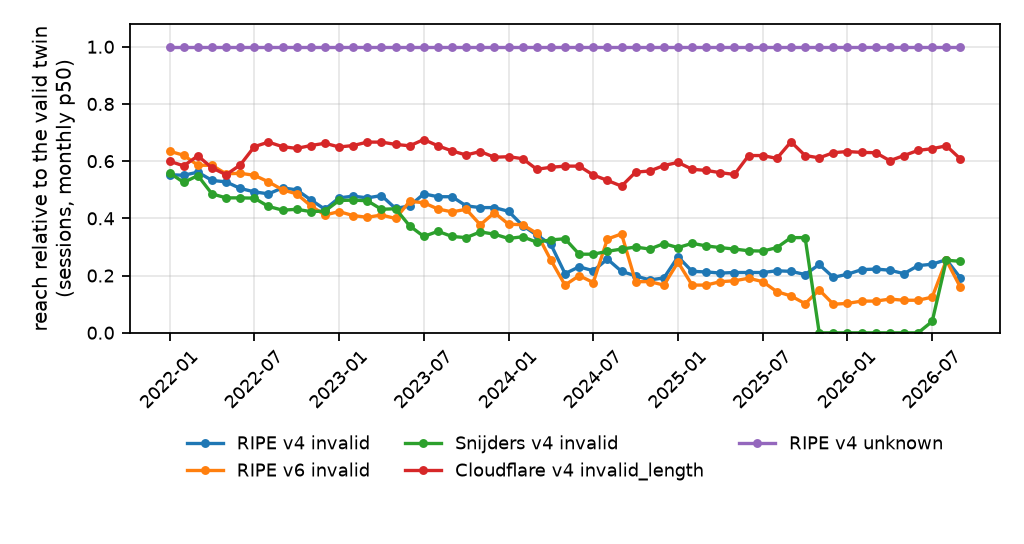
\includegraphics[width=\linewidth]{figures/rpki/beacon_trend}
\caption{Reach of each invalid RPKI beacon relative to the RIPE valid twin: sessions that carry the beacon over sessions that carry the valid twin, per collector snapshot, then the monthly median of these ratios, ten replay collectors, weekly RIBs 2022--2026. The RIPE IPv4 unknown (no-ROA) twin is the reference. Zero reach does not separate withdrawal from filtering.}
\Description{Monthly median beacon reach relative to the valid twin. The RIPE IPv4 invalid series falls from about 0.43 in January 2024 to about 0.21 in May 2024, with two steps in April, and stays near 0.2; the unknown twin stays at 1.0.}
\label{fig:beacons}
\end{figure}

\paragraph{A controlled invalid route.}
We count the peer sessions that carry each beacon prefix in 603 RIB snapshots from 27 collectors.
We divide the reach of each invalid beacon by that of a valid beacon, which removes differences in feed size.
Over all snapshots, the RIPE invalid-origin beacon reaches 0.29 of its valid twin.
The unknown twin reaches the same share of sessions as the valid one (0.363 against 0.362).

Against the RIPE valid twin, the two IPv4 invalid beacons of Snijders reach 0.29 and 0.31.
Against the RIPE valid twin of each address family, the two Cloudflare invalid beacons reach 0.55 and 0.52, in line with earlier reports~\cite{testart2020filter,madory2022kentik,madory2024kentik}.
These beacons have other origins, so their ratios also reflect their origins' upstreams.
% src: docs/paper/corrections-2026-10-16/beacon-independent-verification.json (retained_shares)
% src (round 4, panel-r4 NEW-8 / X1): scripts/beacon_rib_scan.py BEACONS scans no Cloudflare valid prefix; the ratios use the RIPE twins:
%   retained_shares median_share cloudflare_v4_invalid_length 0.200 / ripe_v4_valid 0.362 = 0.55; cloudflare_v6_invalid_asn 0.149 / ripe_v6_valid 0.286
%   = 0.52; snijders 0.106 and 0.111 / 0.362 = 0.29 and 0.31. Origins differ: RIPE AS12654, Snijders AS15562, Cloudflare isbgpsafeyet
%   (beacon_rib_scan.py comments). The former "Against their own valid twins" was wrong.

\paragraph{Trend 2022--2026.}
In 2022--2026, the RIPE IPv4 invalid beacon reaches 0.51, 0.47, 0.22, 0.21 and 0.22 of its valid twin at the ten replay collectors (\Cref{fig:beacons}).
These are yearly medians of the monthly medians.
The monthly median falls from 0.425 in January to 0.207 in May 2024.
The unknown twin is 1.00 in all 57 months, January 2022 to September 2026.
% src: paper/figures/rpki/beacon_trend.csv months 2022-01 .. 2026-09 (57 for RIPE v4 unknown); docs/artifacts-release.md ("beacon snapshots extend
%   through September 2026"). second reviewer round 4, section 5: state the separate beacon end date.

The IPv6 invalid beacon declines from 0.57 in 2022 to 0.12 in 2026.
Its monthly median also falls from 0.390 in March 2024 to 0.286 in April and 0.175 in May, at the time of the IPv4 steps.
% src: paper/figures/rpki/beacon_trend.csv, RIPE v6 invalid ratio_to_valid_p50: 2024-03 0.3902, 2024-04 0.2857, 2024-05 0.175; yearly medians of the
%   monthly medians 2022 0.567, 2026 0.125 (round-3 review NEW-12 / X3: "no single step" removed).
The Snijders IPv4 beacon has zero reach from November 2025 to June 2026 and then returns.
We do not attribute this gap to ROV.

\paragraph{The 2024 drop.}
The monthly median was already 0.342 in March, so about 40\,\% of the fall came before April.
Two weeks give the April steps: 138 to 104 sessions on 2024-04-15, and 105 to 74 on 2024-04-29.
In those weeks, 33 and 30 sessions of 20 and 28 peer ASes dropped the invalid beacon and kept the valid one.
The covering ROAs of both beacons do not change in the four weekly snapshots around these drops.
% src: docs/paper/corrections-2026-10-16/beacon-trend-facts.json; beacon-roa-comparison.json

\paragraph{Which upstream changed.}
In January 2024 the invalid beacon reached our collectors mainly through AS6461 (66 sessions), AS8455 (30), AS8218 (20), AS50673 (17) and AS3320 (14).
On 2024-04-15 AS6461 stopped carrying it, from 75 sessions to none.
On 2024-04-29 AS50673 fell from 54 to 17 sessions.
The total fell by only 34 sessions in the first week, so most sessions moved to other upstreams.
AS6461 never carried the valid twin, so the twin cannot tell ROV at AS6461 from a lost adjacency.

We hold path data for 2024 only, so we cannot say which upstreams explain the later plateau.
RScope reports a similar fall for invalid routes in general~\cite{li2026rscope}.
The share of invalid prefix--origin pairs visible to at least 30\,\% of RouteViews peers fell from 22\,\% in 2023 to 6\,\% in 2025.

\paragraph{Collectors at internet exchange points.}
The beacon ratio varies by collector, from 0.056 at rrc12 to 0.36 at rrc15 in 2024.
We also replayed the 2024 events against Packet Clearing House (PCH) feeds at DE-CIX~\cite{pch_mrt}, from 12--13 of 17 configured sites per day.
Of the \num{1602} selected leaks and \num{18367} selected origin changes of 2024, we exclude 378 and \num{2134} whose PCH window crosses midnight.
Our PCH replay can lose one of the two days of such a window.

PCH observes 35.8\,\% of the remaining \num{1224} leaks and 34.6\,\% of the \num{16233} origin changes.
ASes seen only at PCH form 0.08\,\% of the union for leaks and 0.02\,\% for origin changes.
These IXP feeds therefore add almost nothing to the AS sets of the ten public collectors.
% src: docs/paper/corrections-2026-10-16/beacon-collector-ratios.json; pch/{leak.json,origin.json}
% src: PCH exclusions: docs/paper/corrections-2026-10-16/pch/final-source-verification.json reports (leakpch: selected 1,602, usable 1,224,
%   legacy_crossday_pch_window 378; pchorigin: selected 18,367, usable 16,233, excluded 2,134); pch/README.md (same collector-only file names,
%   so a midnight-spanning window could overwrite one day with the other). Round-3 reviews S10 / second reviewer W6.
%   Round 4 (second reviewer section 5): the denominators are the selected 2024 events (1,602 leaks, 18,367 origin changes), not the 18,350 usable ones.
